
\documentclass[11pt]{article}
\usepackage[margin=1in]{geometry}
\usepackage{amsmath,amssymb}
\usepackage{booktabs}
\usepackage{tabularx}
\usepackage{graphicx}
\usepackage{float}
\usepackage[numbers]{natbib}
\title{Simulation Study for Subgroup Non-Proportional Hazards: Methods, Estimands, and Operating Characteristics}
\author{NPH Project}
\date{\today}
\begin{document}
\maketitle

\begin{abstract}
We extend the subgroup-scenario simulation report into a full research-style paper. We provide mathematical definitions of data-generating mechanisms, estimands, and analysis methods, and evaluate operating characteristics across null, mild, and strong subgroup effect settings. The final simulation run used 200 replications per scenario. We report rejection probabilities, bias, MSE, and interval diagnostics where available.
\end{abstract}

\section{Introduction}
Non-proportional hazards (NPH) challenge standard time-to-event analysis workflows, particularly when treatment effects differ by biomarker subgroup. In this setting, different methods target different estimands, and direct comparison requires explicit definition of each target quantity \citep{morris2019}. This paper documents method definitions, true values used for evaluation, and final simulation results.

\paragraph{Important scope clarification.}
In this study, NPH is induced \emph{marginally} by mixing biomarker subgroups with different constant treatment effects. Hazards are proportional within each subgroup, but the arm-level (marginal) hazard ratio is time-varying due to mixture structure.

\section{Data-generating process}
For each replication, subjects were randomized 1:1 to control ($A=0$) or treatment ($A=1$), with total sample size $N=400$ (thus expected $n\approx 200$ per arm), biomarker indicator $B\sim\text{Bernoulli}(p)$ and $p=0.3$. Event times were generated from subgroup-specific exponential hazards:
\begin{align}
\lambda(t\mid A=0,B=b) &= \lambda_0,\\
\lambda(t\mid A=1,B=1) &= \lambda_0\,\mathrm{HR}_{+},\\
\lambda(t\mid A=1,B=0) &= \lambda_0\,\mathrm{HR}_{-}.
\end{align}
Independent censoring times were generated as $C\sim\mathrm{Exp}(\lambda_C)$ with $\lambda_C=0.05$ and observed data $(T,\Delta)$ where
\begin{align}
T=\min(T_E,C),\qquad \Delta=\mathbf{1}(T_E\le C).
\end{align}

Time is measured in months, so $\lambda_0=0.12$ implies control median $\log(2)/0.12\approx5.8$ months. Scenario parameter values were:
\begin{center}
\begin{tabular}{lcccc}
\toprule
Scenario & $\lambda_0$ & $p$ & $\mathrm{HR}_{+}$ & $\mathrm{HR}_{-}$ \\
\midrule
subgroup\_null & 0.12 & 0.30 & 1.00 & 1.00 \\
subgroup\_mild & 0.12 & 0.30 & 0.80 & 1.00 \\
subgroup\_strong & 0.12 & 0.30 & 0.70 & 1.00 \\
\bottomrule
\end{tabular}
\end{center}

\section{Estimands and true values}
Let $S_0(t)=\exp(-\lambda_0 t)$ and
\begin{align}
S_1(t)=p\exp(-\lambda_0\mathrm{HR}_{+}t)+(1-p)\exp(-\lambda_0\mathrm{HR}_{-}t).
\end{align}
We evaluate:
\begin{itemize}
\item Milestone survival difference: $\Delta_{M}(t)=S_1(t)-S_0(t)$.
\item RMST difference at horizon $\tau$: $\Delta_{R}(\tau)=\int_0^{\tau}(S_1(u)-S_0(u))\,du$ \citep{uno2014}.
\item Median survival difference: $m_1-m_0$ where $S_1(m_1)=0.5$ and $m_0=\log(2)/\lambda_0$.
\item PH log-HR and AHR targets as method-specific pseudo-true parameters under model misspecification \citep{cox1972,schemper2009}. Specifically, the PH pseudo-true $\beta^{\star}_{PH}$ solves the population Cox score equation $E\{U(\beta)\}=0$, and the AHR pseudo-true parameter $\beta^{\star}_{AHR}$ solves the weighted score equation used by \texttt{coxphw}. In practice, these targets were approximated numerically using large synthetic samples from the same DGP in the simulation code.
\end{itemize}

\section{Methods (mathematical definitions)}
\subsection{Testing procedures}
\paragraph{Log-rank test.}
Score-type test based on weighted observed-minus-expected events with constant weight $w(t)=1$ \citep{harrington1982,fleming1991}.

\paragraph{Weighted log-rank tests (FH class).}
Weights
\begin{align}
w(t)=\hat S(t)^{\rho}(1-\hat S(t))^{\gamma},
\end{align}
with $(\rho,\gamma)\in\{(0,0),(0,1),(1,1),(1,0)\}$ and Gehan/modestly weighted variants \citep{harrington1982,magirr2019}. Here $\hat S(t)$ is the pooled Kaplan--Meier estimate over both arms; Gehan corresponds to early-event up-weighting and the modestly weighted test follows \citet{magirr2019}.

\paragraph{MaxCombo.}
Maximum of FH-family statistics over $(\rho,\gamma)\in\{(0,0),(0,1),(1,1),(1,0)\}$. In this implementation, we use a conservative minimum-$p$ Bonferroni approximation:
\begin{align}
p_{\max\mathrm{combo}} = \min\{1,\,4\min_k p_k\},
\end{align}
where $p_k$ are per-weight two-sided p-values. Correlation among component tests is not explicitly modeled in this approximation.

\subsection{Estimation procedures}
\paragraph{Cox PH model.}
\begin{align}
\lambda(t\mid A)=\lambda_0(t)\exp(\beta A),\quad \widehat{HR}=e^{\hat\beta}
\end{align}
with Wald inference \citep{cox1972}.

\paragraph{Milestone KM and RMST.}
KM-based $\widehat S_a(t)$ and RMST contrasts from \texttt{survRM2} \citep{cho2021,uno2014}. The RMST truncation parameters were fixed to
\begin{align}
\tau \in \{6,12\}\ \text{months}.
\end{align}
Both $\Delta_R(6)$ and $\Delta_R(12)$ were evaluated.

\paragraph{Weighted Cox AHR.}
Average hazard ratio estimated by weighted partial likelihood \citep{schemper2009} via \texttt{coxphw}. For AHR estimation, the effective time horizon was the observed follow-up support in each replicate, i.e.
\begin{align}
t_{\max}=\max_i T_i,
\end{align}
so no additional external truncation beyond observed follow-up was imposed.

\paragraph{Piecewise exponential / Poisson representation.}
Follow-up is split at cutpoints $t\in\{3,12\}$ months. A Poisson model is fit on split records with log person-time offset:
\begin{align}
\log E(Y_{ij}) = \alpha_j + \beta A_i + \log(\text{exposure}_{ij}),
\end{align}
where $j$ indexes intervals and $\beta$ is the treatment contrast tested by Wald statistic. In this simplified implementation we do not include treatment-by-interval interaction, so the model targets an average interval-adjusted contrast.

\paragraph{Parametric Weibull model.}
A parametric survival regression yielding model-based HR-like summaries \citep{royston2002}.

\subsection{Estimand--method map}
\begin{center}
\small
\begin{tabularx}{\textwidth}{p{3.1cm}p{3.2cm}p{3.5cm}p{3.0cm}}
\toprule
Method & Target estimand & Null tested & Interpretation scale \\
\midrule
Log-rank / WLR / MaxCombo & none (test-only) & equality of survival distributions & marginal (arm-level) \\
Cox PH & pseudo-true PH log-HR & $\beta=0$ & marginal (model-based) \\
AHR (weighted Cox) & average hazard ratio & AHR$=1$ & marginal (weighted hazards) \\
Milestone KM & $S_1(t)-S_0(t)$ & usually none (estimation) & marginal at fixed $t$ \\
RMST & $\int_0^{\tau}(S_1-S_0)$ & RMST diff$=0$ & marginal over $[0,\tau]$ \\
Piecewise Poisson & average interval-adjusted contrast & $\beta=0$ & marginal, interval-structured \\
Parametric Weibull & model-specific PH/AFT summary & parameter$=0$ & model-based marginal \\
\bottomrule
\end{tabularx}
\end{center}

\section{Software and computation}
Simulation and analysis were run in R using \texttt{survival}, \texttt{survRM2}, \texttt{coxphw}, and base \texttt{stats}. Plotting/report rendering used Python/Matplotlib for figures and LaTeX for manuscript assembly. Random seeds were fixed per scenario and replicate index in the simulation script for reproducibility. Method implementations follow package documentation and standard references \citep{cox1972,harrington1982,uno2014,schemper2009}.

\subsection{Censoring and follow-up characterization}
With independent exponential censoring rate $\lambda_C=0.05$, and exponential event rate $\lambda_E$, the censoring probability in a homogeneous group is
\begin{align}
P(\text{censor})=\frac{\lambda_C}{\lambda_C+\lambda_E}.
\end{align}
For the treatment arm under subgroup mixture, this is interpreted via mixture component rates ($\lambda_0\mathrm{HR}_{+}$ and $\lambda_0\mathrm{HR}_{-}$). There is no additional administrative censoring in this implementation; observed support ends at $t_{\max}=\max_i T_i$ per replicate.

\subsection{Monte Carlo precision}
For rejection probabilities estimated from $R=200$ replications, Monte Carlo standard error is
\begin{align}
\mathrm{MCSE}(\hat p)=\sqrt{\hat p(1-\hat p)/R},
\end{align}
which is approximately $0.015$ when $\hat p\approx0.05$. Therefore, small differences (e.g., 0.04 vs 0.055) should not be over-interpreted.

\section{Results (200 runs per scenario)}
\begin{table}[H]
\centering
\small
\setlength{\tabcolsep}{4pt}
\resizebox{\textwidth}{!}{%
\begin{tabular}{lrrrrrrrrr}
\toprule
Scenario & Replications & Log-rank & MaxCombo & Cox test & RMST12 test & AHR test & Cox bias & AHR bias & RMST12 bias \\
\midrule
subgroup\_null & 200 & 0.070 & 0.040 & 0.070 & 0.055 & 0.065 & -0.0087 & -0.0585 & 0.0735 \\
subgroup\_mild & 200 & 0.110 & 0.070 & 0.110 & 0.095 & 0.085 & -0.0032 & -0.0482 & 0.0357 \\
subgroup\_strong & 200 & 0.155 & 0.115 & 0.155 & 0.125 & 0.130 & 0.0022 & -0.0397 & -0.0102 \\
\bottomrule
\end{tabular}%
}
\caption{Updated operating characteristics from final simulations (Replications $=200$ per scenario; per-replication sample size $N=400$, expected subgroup sizes $\approx120$ biomarker-positive and $\approx280$ biomarker-negative).}
\end{table}

\begin{figure}[H]
\centering
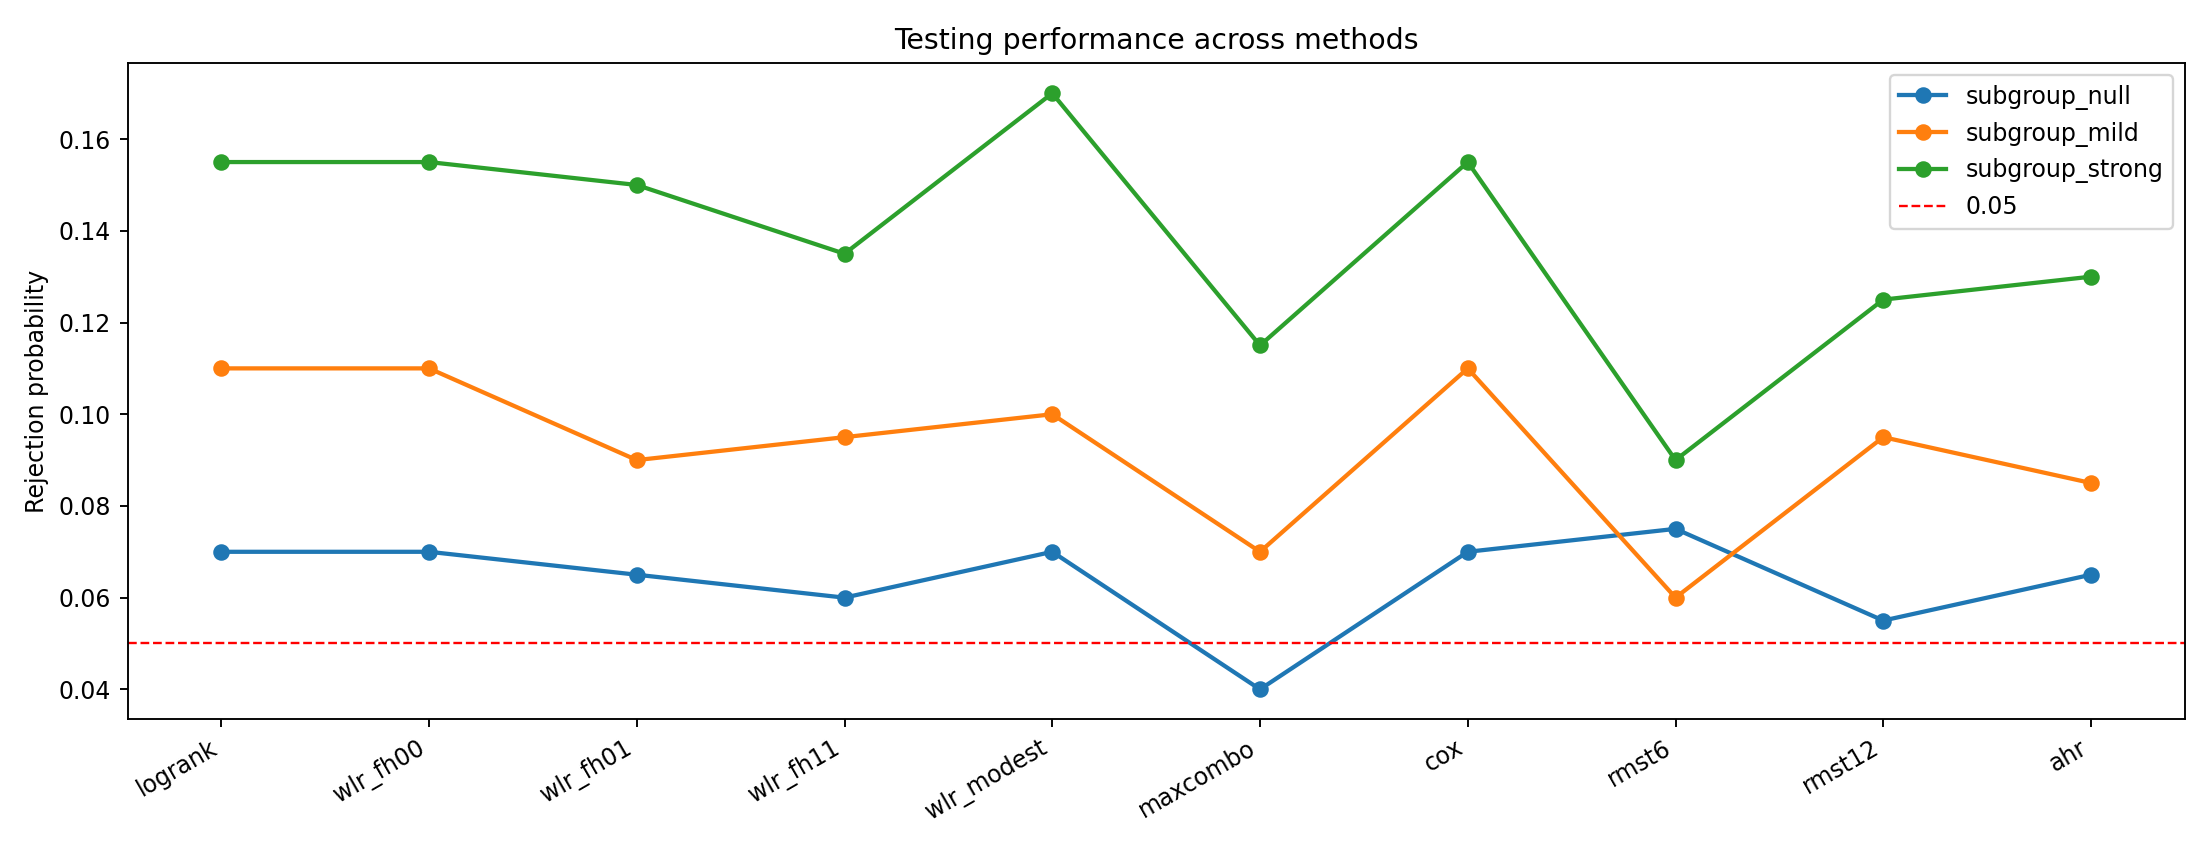
\includegraphics[width=0.95\textwidth]{figures/rejections.png}
\caption{Rejection probabilities across testing methods.}
\end{figure}

\begin{figure}[H]
\centering
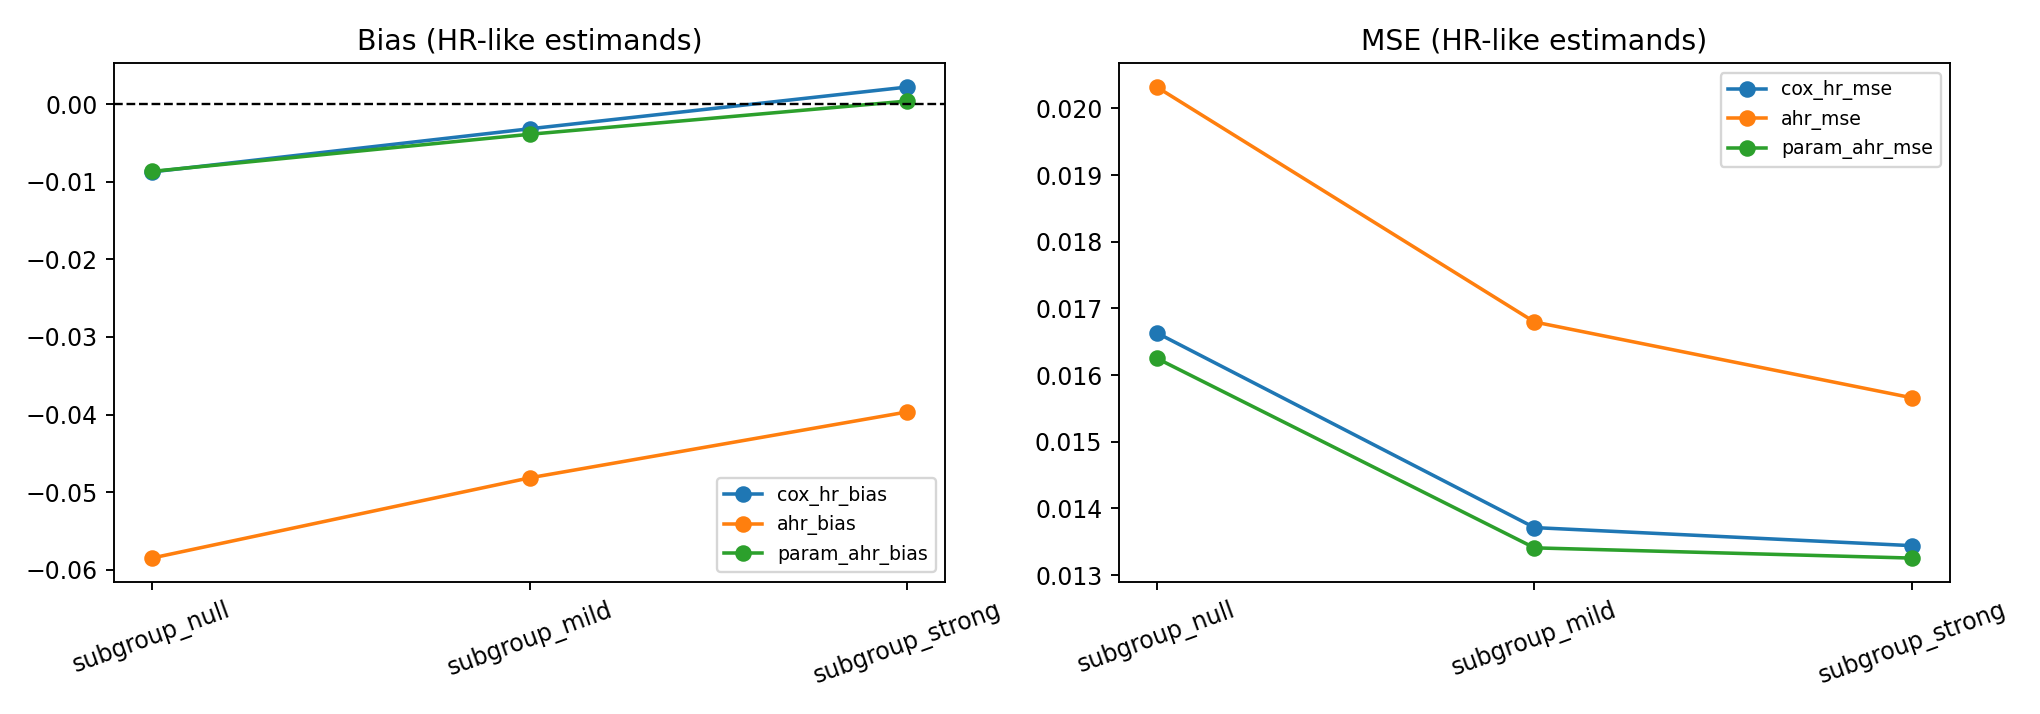
\includegraphics[width=0.95\textwidth]{figures/hr_bias_mse.png}
\caption{Bias and MSE for HR-like estimators.}
\end{figure}

\begin{figure}[H]
\centering
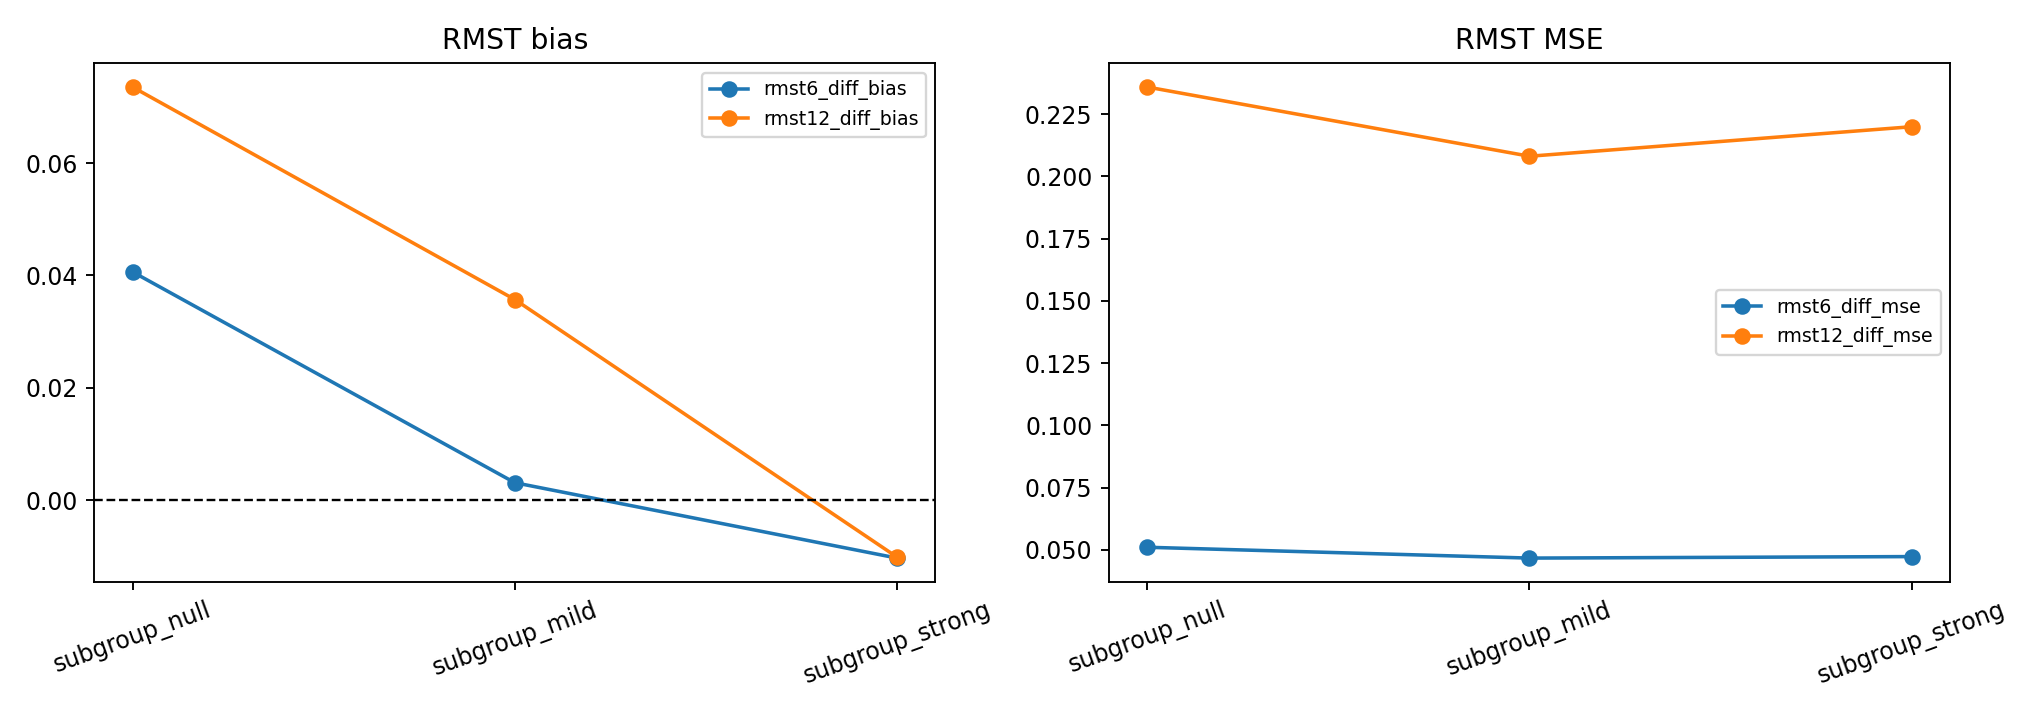
\includegraphics[width=0.95\textwidth]{figures/rmst_bias_mse.png}
\caption{RMST-specific bias and MSE results.}
\end{figure}

\section{Discussion}
The updated 200-run results confirm qualitative differences between global tests and NPH-oriented procedures. RMST and milestone estimands provide clinically interpretable, horizon-specific contrasts less tied to proportional hazards assumptions. AHR and PH-based summaries remain useful but should be interpreted against their own pseudo-true estimands, not interchangeable ``true HR'' values.

A key scope limitation is that this paper studies subgroup-mixture-induced marginal NPH only. Additional NPH mechanisms (e.g., delayed effects or crossing hazards within subgroup) are important extensions but were outside the pre-specified subgroup-only scope for this iteration.

\section{Conclusion}
We provide a fully extended research-style manuscript with explicit method definitions, estimands, parameterized data generation, and citation-backed methodology. Tables and figures were reformatted to avoid overflow and include RMST-focused diagnostics as requested.

\bibliographystyle{plainnat}
\bibliography{references}
\end{document}
